\documentclass{report}
\usepackage{ifxetex}
\usepackage[svgnames]{xcolor}
\ifxetex{%
  \usepackage{fontspec}
  \setmainfont{Linux Libertine O} % or any font on your system
  \newfontfamily\quotefont[Ligatures=TeX]{Linux Libertine O} % or any font on your system
\else
  \usepackage[utf8]{inputenc}
  \usepackage[T1]{fontenc}
  \usepackage{libertine} % or any other font package (or none)
  \newcommand*\quotefont{\fontfamily{fxl}} % selects Libertine for quote font
\fi
\usepackage{tikz}
\usepackage{framed}
\usepackage{hyperref}

% Make commands for the quotes
\newcommand*{\openquote}{\tikz[remember picture,overlay,xshift=-15pt,yshift=-10pt]
     \node (OQ) {\quotefont\fontsize{30}{30}\selectfont``};\kern0pt}
\newcommand*{\closequote}{\tikz[remember picture,overlay,xshift=15pt,yshift=10pt]
     \node (CQ) {\quotefont\fontsize{30}{30}\selectfont''};}
% select a colour for the shading
\definecolor{shadecolor}{named}{Azure}
% wrap everything in its own environment
\newenvironment{shadequote}%
{\begin{snugshade}\begin{quote}\openquote}
{\hfill\closequote\end{quote}\end{snugshade}}

\begin{document}
\section*{Introduction}
The over all aim of the project is to investigate means of measuring the explicitness of language in textual documents using the keyword density mertric. This report will detail the progress to date on S.T.E.L.A framework (Strathclyde Toolkit for Explicit Language Analysis). 
\section*{Progress since the poster day}
After my presentation at the poster day on Feburary 6th Dr Weir had recommended I look in to the concept of "Ngram Generation" in order to aid with issues I had mentioned with the multi-term frequency calculations. After a little background reading on the subject i had set to work on generating the possible Ngrams for the dataset (or black list). The biggest issue that occurred during the development of these Ngrams has been described below.
\begin{description}
\item[Concurrent Access Exceptions]
In order to generate the algorithms in a relativley memory efficient way I constantly read from file, modify the line and then write it back. In a vain attempt at speeding up the process I decided to use a multi-threaded approach to this aspect of the application, which caused access violations as each thread began to access the file at the same time. In order to fix this issue, I abanonded the multi-threaded approach and made a slightly more elegant single threaded approach duplicating the black list stored in memory and modifying the duplicate. In hindsight I could have adoped the use of semaphores, I do however believe the technique currently in operation is also an efficient method of generation.
\end{description}

\section*{N-grams}
Generating N-grams is the process of creating all possible combinations of words in a dataset. In terms of this project this involved taking the blacklist (dictionary of explicit words and phrases) and generating all possible combinations of these words. This proved interesting as although many of the combinations made little to no gramatical sense, many of the generations prove to be extremely explicit and in fact made sense in the correct context.
\\
By generating these N-grams i have been able to factor in some basic contextual understanding of language into the framework by allowing the multi-word search to operate with the N-grams as a data set rather than exclusivley the blacklist itself.
\\
\\
\section*{Lemmatization}
Whilst researching the area called stemming I came across the technique of lemmatization a process which involves grouping (or clusering) together different forms of a words to allow them to be analysed as a single term. This approach has proven to be extremely positive in terms of this project with the dataset i have chosen to work with as during the implementation of the basic word frequency analysis different spellings of the same word would often appear in much higher quantities than the correctly spelled word alone.
\\
\\
Stemming can also be used in this process to ensure that if the word exists in a variation not specified by the lemmatizer it can still be found.
\\
\\

In order to build this technique into the framework I have designed and specified a file structure "SWDL" which involves using a single word (the associated word) followed by a colon with variations of the word defined after the colon. After which the corpa is fed into the lemmatizer which replaces each variation with the associated word. This techniqued has yielded some excellent results when combined with the basic frequency analyzer and has improved upon the keyword density scores for each document.

\section*{Sentiment Analysis}
Another technique I have spent much time researching is the area of sentiment analysis. Sentiment analysis is an active research area within the realms of compuational linguistics and information retrieval used to identify and extract subjective information from relevant corpa. 
\\
I feel that current area's of research into sentiment analysis (such as capturing favorability) will provide a good starting ground for expanding the area into functionality within the realm of sexually explicit material. By modifying existing algorithms, I believe it will be possible to modify the targeted material from favorability to sexually explicit material using existing algorithms.

\section*{Addressing the second assessors comments}
Below is a list of the recommendations made by my second assessor and how i have addressed them.
\begin{shadequote}
At this stage I would recommend the production of a draft background and related works chapter to get this out of the way and also to inform/measure future development.
\end{shadequote}
As suggested i have begun to draft a report on specific areas of background reading, as well as the use of Mendeley Desktop to keep track of which papers are being used as reference.
\\
\begin{shadequote}
A number of design and implementation decisions still need to be pinned down and it’s important that this is done without undue delay since the final product will need to demonstrate some novelty and innovation.
\end{shadequote}
In order to address design issues i have written the package as a toolkit (S.T.E.L.A ~ The Strathclyde Toolkit for Explicit Language Analysis) allowing for use with any other applications. This also allows a speedy development of a front end in terms of the project.
\\
\begin{shadequote}
Likewise, a good evaluation strategy will need to be adopted and results from this analysed to produce a valid comparison with other, related, systems. Ethics approval needs also to be sorted out ASAP given the nature of the project.
\end{shadequote}
In terms of evaluation I have made good progress towards the preparation for tests. I have received ethics approval from the department and I aim to carry out the experiment by the week ending the 8'th of March, leaving me a little over two weeks to write the evaluation report and compare the results. Also following the seminar presented by Dr Dunlop, I have created an excel spreadsheet for gathering data from the experiments a copy of which can be found at \url{https://github.com/chris-forbes-1/measuring_content/blob/Experimental/Experiment Calculations.xlsx}
\\
\section*{Next steps}
As discussed at the poster day, the next step will be to add weights to the blacklist words (the dictionary of explicit words used for analysis). To do this i will firstly lemmatize the words from the corpa, by defining a file  I am also aiming to impliment a modified version of the sentiment analysis described in 'Sentiment analysis: Capturing favorability using natural language processing by Tetsuya Nasukawa and Jeonghee Yi'.

\section*{Alterations to project plan}
Very few alterations have been made to the project plan. I have added a separate step into the project plan to account for the inclusion of sentiment analysis in to the toolkit.
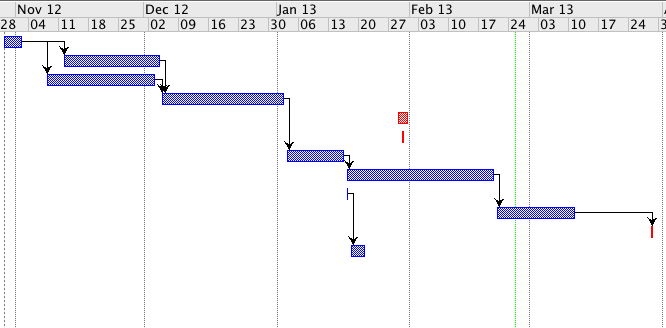
\includegraphics[scale=0.5]{ProjPlan.png}
\end{document}
